
%% bare_conf.tex
%% V1.3
%% 2007/01/11
%% by Michael Shell

\documentclass[conference]{IEEEtran}

\usepackage{booktabs}
\usepackage{tikz}
\usepackage{url}
\usepackage{pdfpages}
\usepackage{afterpage}
\usepackage{color, colortbl}
\usepackage{graphicx} 
\usepackage{amsmath}
\usepackage{subfigure}
\usepackage{footmisc}
\usepackage{epstopdf}
\usepackage{etoolbox}
\graphicspath{{./figures/}}
%\usepackage{caption}% http://ctan.org/pkg/caption
%\captionsetup[table]{justification=centering,font={sc,small}}%


%\makeatletter
%%\patchcmd{\@makecaption}
%%{\scshape}
%%{}
%%{}
%%{}
%%\makeatletter
%\patchcmd{\@makecaption}
%{\\}
%{.\ }
%{}
%{}
%\makeatother
%\def\tablename{Table}

\begin{document}

\begin{figure*}[h]
	\centering     %%% not \center
	\subfigure[Performance (GFlops)]
	{
		\includegraphics[width=0.48\linewidth]{perf_winograd.eps}
	}
	\subfigure[Power (Watt)]
	{
		\includegraphics[width=0.48\linewidth]{power_winograd.eps}
	}
	\caption{\label{fig:pp_winograd} Performance and power consumption of convolution on Nvidia GTX 980 with DVFS. GPU core frequency ranges from 600 MHz to 1300 MHz; GPU memory frequency ranges from 2100 MHz to 3800 MHz.}
\end{figure*}

\begin{figure*}[h]
	\centering     %%% not \center
	\subfigure[Performance (time per iteration in seconds)]
	{
		\includegraphics[width=0.48\linewidth]{perf_fcn.eps}
	}
	\subfigure[Power (Watt)]
	{
		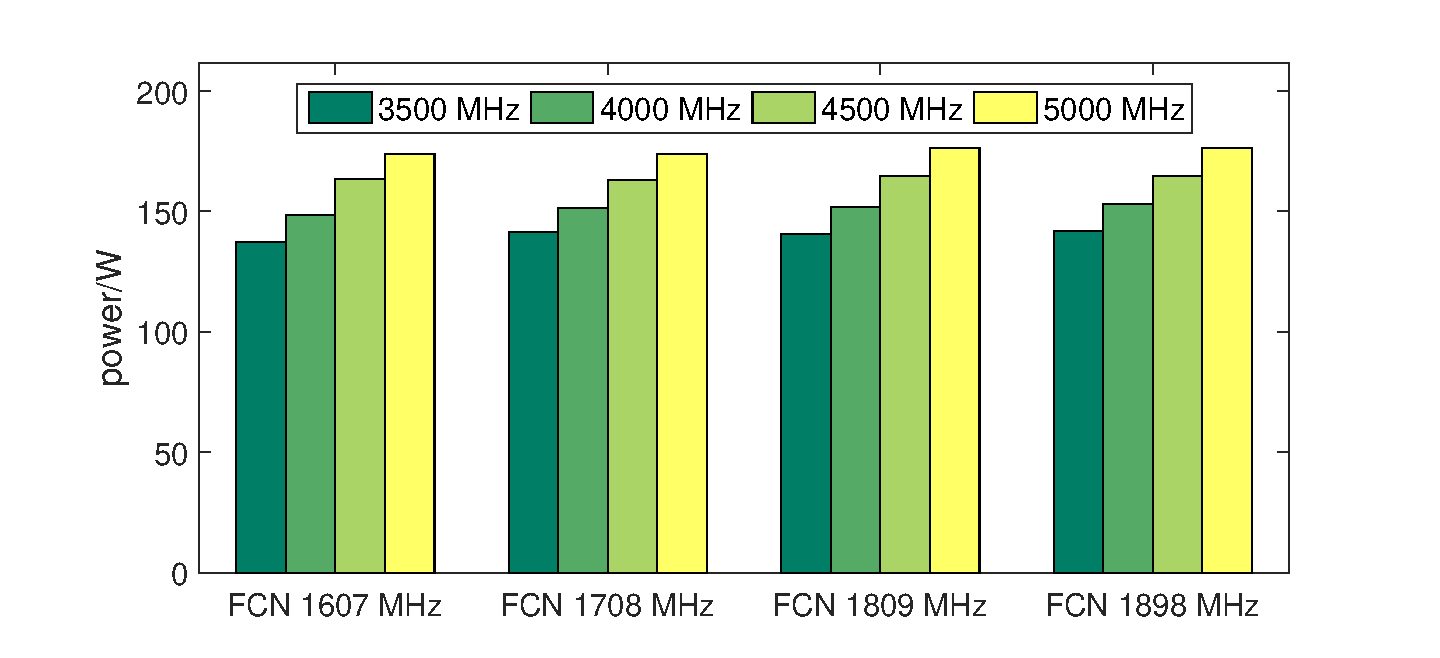
\includegraphics[width=0.48\linewidth]{power_fcn.eps}
	}
	\caption{\label{fig:pp_fcn} Performance and power consumption of training a fully-connected neural network on Nvidia GTX Titan X with DVFS. GPU core frequency ranges from 1607 MHz to 1898 MHz; GPU memory frequency ranges from 3500 MHz to 5000 MHz.}
\end{figure*}	
	


% that's all folks
\end{document}


